%!TEX encoding = UTF-8 Unicode
% $Id: 25-object-oriented_lisp.tex 18 2014-03-12 22:35:24Z binghe $

\chapter{面向对象的~Lisp}
\label{chap:object-oriented_lisp}

本章讨论了~Lisp 中的面向对象编程。Common Lisp 提供了一组操作符可供编写
面向对象的程序时使用。这些操作符和起来,并称为~Common Lisp Object
System\index{Common Lisp Object System|see{\textsc{clos}}},或者叫~CLOS。在这里我们不把~CLOS 仅仅看作一种编写面向对象程序的
手段,而把它本身就当成一个~Lisp 程序。从这个角度来看待~CLOS 是理
解~Lisp 和面向对象编程之间关系的关键。

\section[万变不离其宗]{万变不离其宗\protect \footnote{译者注:在原文
    中,本节的标题是~``Plus ça Change''。它源自法国谚语~``plus ça
    change, plus c'est la même chose'',字面意思是:变化得越多,
    越是原来的事物。平时使用中常常略作前半句。}}
\label{sec:plus_ca_change}

面向对象的编程意味着程序组织方式的一次变革。历史上的另一个变化与这个变
革有几分类似,即发生在处理器计算能力分配方式上的变化。在~1970 年代,多用
户计算机系统指的就是联接到大量哑终端\footnote{译者注:指和常用的工作站相
  比,功能较有限的计算机终端。}的一两个大型机\index{mainframes 大型机}。
时至今日,这个词更
有可能说的是大量用网络互相联接的工作站\index{workstations}。现在,系统的处理能力散布于多个
独立用户中,而不是集中在一台大型计算机上。

这与面向对象编程有很大程度上的相似\index{object-oriented programming!like distributed systems},后者把传统的程序结构拆分开来:它不再让单一的程序逻辑去操纵那些被动的数据,而是让数据自己知道该做些什
么,程序逻辑就隐含在这些新的数据``对象''间的交互过程之中。

举例来说,假设我们要算出一个二维图形的面积。解决这个问题的一个办法就是
写一个单独的函数,让它检查参数的类型,然后分情况处理:
\begin{lstlisting}
(defun area (x)
  (cond ((rectangle-p x) (* (height x) (width x)))
        ((circle-p x) (* pi (expt (radius x) 2)))))
\end{lstlisting}

面向对象的方法则是让每种对象自己就能够计算出自身的面积。\texttt{area}
这个函数就被拆开,同时每条语句都被分到对象的对应类型中去,比
如~\texttt{rectangle} 类可能就会看起来像这样
\begin{lstlisting}
#'(lambda (x) (* (height x) (width x)))
\end{lstlisting}
至于~\texttt{circle} 则会是这样
\begin{lstlisting}
#'(lambda (x) (* pi (expt (radius x) 2)))
\end{lstlisting}
在这种模式下,我们向对象询问该对象的面积,然后对象则根据所属类型所提供
的方法来作出回应。

CLOS 的到来似乎意味着~Lisp 正在改变自己,以拥抱面向对象的编程方式。与其
这样说,不如改成:Lisp 还在墨守成规,用老样子来拥抱面向对象编程,这样
还确切一些。不过~Lisp 中的那些基本概念没有名字\index{object-oriented programming!name of},\note{349}面向对
象编程却有,所以时下有种趋势要把~Lisp 算成面向对象的语言。另一种说
法:Lisp 是一门可扩展的语言,在这种语言里,面向对象编程的机制和结构可以
轻松实现,这种说法恐怕更接近真相。

由于~CLOS 是原来就有的,所以把~Lisp 说成面向对象的编程语言并没有误导。
然而,如果就这样看待~Lisp 未免太小觑它了。诚然,Lisp 是一种面向对象的编
程语言,但是原因并不是它采纳了面向对象的编程模式。事实在于,这种编程模
式只是~Lisp 的抽象系统提供的又一种可能性而已。为了证明这种可能性,我们
有了~CLOS \pozhehao{} 一个~Lisp 程序,它让~Lisp 成为了一门面向对象的语
言。

本章的主旨在于:通过把~CLOS 作为一个嵌入式语言\index{CLOS@\textsc{clos}!as an embedded language}的实例来研究,进而揭
示~Lisp 和面向对象编程之间的联系。这同时也是了解~CLOS 本身的一个很好的
手段,要学习一个编程语言的特性,没什么方法能比了解这个特性的实现更有效
的了。在第~\ref{sec:a_model_of_macros} 节,那些宏就是用这种方式来讲解的。
下一节将会有一个类似的对面向对象抽象是如何建立在~Lisp 之上的一个粗略的
介绍。其中提到的程序将被第~\ref{sec:classes_and_instances} 节到
第~\ref{sec:auxiliary_methods_and_combination} 节作为一个基准实现来
参考。

\section{阳春版~Lisp 中的对象}
\label{sec:objects_in_plain_lisp}
\index{object-oriented programming!in plain Lisp}

我们可以用~Lisp 来模拟各种各样不同种类的语言\index{Lisp!defining features of}。有一种特别直接的办法可以
把面向对象编程的理念对应到~Lisp 的基本抽象机制上。不过,CLOS 的庞大规模
让我们难以认清这个事实。因此,在我们开始了解~CLOS 能让我们做什么之前,
不妨先看看我们用最原始的~Lisp 都能干些什么。

我们在面向对象编程中想要的大多数特性,其实在~Lisp 里面已经有了。我们可
以用少得出奇的代码来得到剩下的那部分。在本节中,我们将会用两页纸的代码
实现一个对象系统,这个系统对于相当多真实的应用已经够用了。面向对象编
程,简而言之,就是\index{object-oriented programming!defining features of}:
\begin{enumerate}
\item 具有属性的对象
\item 它能对各种消息作出反应,
\item 而且对象能从它的父对象继承相应的属性和方法。
\end{enumerate}

在~Lisp 里面已经有好几种存放成组属性的方法。其中一种就是把对象实现成哈
希表\index{hash tables 哈希表},把对象的属性作为哈希表里的表项。这样我们就可以用~\texttt{gethash} 来访问指定的属性:
\begin{lstlisting}
(gethash 'color obj)
\end{lstlisting}
由于函数是数据对象,我们同样可以把它们当作属性保存起来。这就是说,我们
的对象系统也可以有方法了,要调用对象的特定方法就~funcall 一下哈希表里的
同名属性:
\begin{lstlisting}
(funcall (gethash 'move obj) obj 10)
\end{lstlisting}
据此,我们可以定义一种~Smalltalk\index{Smalltalk} 风格的消息传递\index{message-passing 消息传递}语法:
\begin{lstlisting}
(defun tell (obj message &rest args)
  (apply (gethash message obj) obj args))
\end{lstlisting}
这样的话,要告诉~(tell)~obj 移动~10 个单位,就可以说
\begin{lstlisting}
(tell obj 'move 10)
\end{lstlisting}

事实上,阳春版~Lisp 唯一缺少的要素就是继承机制,不过我们可以用六行代码
来实现一个初步的版本,这个版本用一个递归版的~\texttt{gethash}\index{gethash@\texttt{gethash}!recursive version} 来完成这
个功能:
\begin{lstlisting}
(defun rget (obj prop)
  (multiple-value-bind (val win) (gethash prop obj)
    (if win
        (values val win)
        (let ((par (gethash 'parent obj)))
          (and par (rget par prop))))))
\end{lstlisting}
如果我们在原本用~\texttt{gethash} 的地方用~\texttt{rget},就会得到继承而来的属性和方法。如此这般,就可以指定对象的父类:
\begin{lstlisting}
(setf (gethash 'parent obj) obj2)
\end{lstlisting}
到现在为止,我们只是有了单继承\pozhehao{}即一个对象只能有一个父类。不过我
们可以把~\texttt{parent} 属性改成一个列表,这样就能有多继承了,如
图~\ref{fig:multiple_inheritance} 中定义的~\texttt{rget}。

\begin{figure}
\begin{lstlisting}
(defun rget (obj prop)
  (some2 #'(lambda (a) (gethash prop a))
         (get-ancestors obj)))

(defun get-ancestors (obj)
  (labels ((getall (x)
             (append (list x)
                     (mapcan #'getall
                             (gethash 'parent x)))))
    (stable-sort (delete-duplicates (getall obj))
                 #'(lambda (x y)
                     (member y (gethash 'parents x))))))

(defun some2 (fn lst)
  (if (atom lst)
      nil
      (multiple-value-bind (val win) (funcall fn (car lst))
        (if (or val win)
            (values val win)
            (some2 fn (cdr lst))))))
\end{lstlisting}
\caption{\label{fig:multiple_inheritance}多继承}
\index{inheritance!multiple!sketch of}
\end{figure}

在单继承体系里面,当我们需要得到对象的某个属性时,只需要递归地在对象的
祖先中向上搜索。如果在对象本身里面没有我们想要的属性信息时,就检查它的
父类,如此这般直到找到。在多继承体系里,我们一样会需要做这样的搜索,但
是这次的搜索会有点复杂,因为对象的多个祖先会构成一个图,而不再只是个简
单列表了。我们不能用深度优先来搜索这个图。如果允许有多个父类,我们有如
图~\ref{fig:multiple_paths_to_a_superclass} 中所示的继承树:\texttt{a} 继承
自~\texttt{b} 和~\texttt{c},而~\texttt{b} 和~\texttt{c} 均继承于~\texttt{d}。深度优
先~(或叫高度优先) 的遍历会依次走过~\texttt{a}、\texttt{b}、\texttt|d|、\texttt{c}
和~\texttt{d}。倘若想要的属性同时存在于在~\texttt{d} 和~\texttt{c} 里,
那么我们将会得到~\texttt{d} 中的属性,而非~\texttt{c} 中的。这种情况
会违反一个原则:即子类应当会覆盖基类中提供的缺省值。
\begin{figure}
\begin{center}
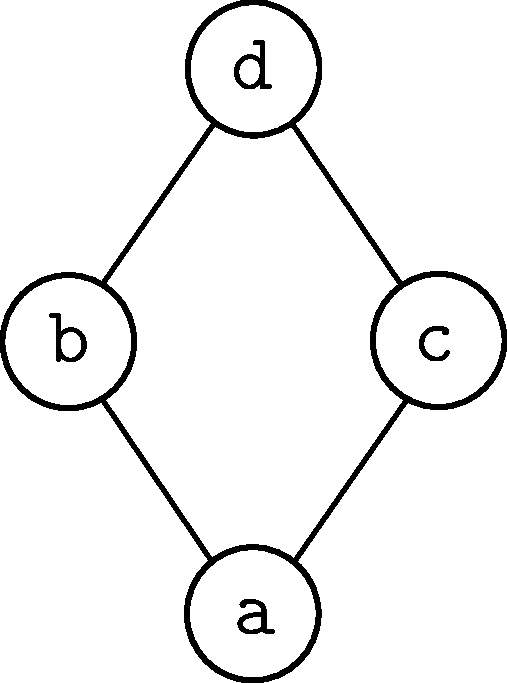
\includegraphics[width=.18\textwidth]{multi-inheritance.pdf}
\end{center}
\caption{\label{fig:multiple_paths_to_a_superclass}到同一基类的多条路径}
\end{figure}

如果需要实现继承系统的基本理念,我们就绝不能在检查一个对象的子类之
前,提前检查该对象。在本例中,正确的搜索顺序应该是~\texttt{a}、\texttt{b}、
\texttt{c}、\texttt{d}。那怎么样才能保证搜索的顺序是先尝试子孙再祖先呢?
最简单的办法是构造一个列表,列表由原始对象的所有祖先构成,然后对列表排序,
让列表中没有一个对象出现在它的子孙之前,最后再依次查看每个元素。

\texttt{get-ancestors} 采用了这种策略,它会返回一个按照上面规则排序的列
表,列表中的元素是对象和它的祖先们。\note{352}为了避免在排序时把同一层
次的祖先顺序打乱,\texttt{get-ancestors} 使用的是~\texttt{stable-sort}\index{stable-sort@\texttt{stable-sort}}\index{sorting|seealso {stable-sort@\texttt{stable-sort}}}
而非~\texttt{sort}\index{sort@\texttt{sort}}。一旦排序完毕,\texttt{rget} 只要找到第一个具有期望
属性的对象就可以了。(\utility~\texttt{some2} 是~\texttt{some} 的一个修
改版,它能适用于~\texttt{gethash} 这类用第二个返回值表示成功或失败的函数。)

对象的祖先列表中元素的顺序是先从最具体的开始,最后到最一般的类型。如
果~\texttt{orange} 是~\texttt{citrus} 的子类型,后者又
是~\texttt{fruit} 的子类型,那么列表的顺序就会像这样:\texttt{(orange
  citrus fruit)}。

% pp252
倘若有个对象,它具有多个父类,那么这些前辈的座次会是从左到右排列的。也就是
,如果我们说
\begin{lstlisting}
(setf (gethash 'parents x) (list y z))
\end{lstlisting}
那么当我们在搜索一个继承得来的属性时,\texttt{y} 就会优先于~\texttt{z}
被考虑。举个例子,我们可以说爱国的无赖\index{scoundrels, patriotic}首先是一个无赖,然后才是爱国者:
\begin{lstlisting}
> (setq scoundrel (make-hash-table)
        patriot (make-hash-table)
        patriotic-scoundrel (make-hash-table))
#<Hash-Table C4219E>
> (setf (gethash 'serves scoundrel) 'self
        (gethash 'serves patriot)   'country 
        (gethash 'parents patriotic-scoundrel)
                 (list scoundrel patriot))
(#<Hash-Table C41C7E> #<Hash-Table C41F0E>)
> (rget patriotic-scoundrel 'serves)
SELF
T
\end{lstlisting}

现在让我们对这个简陋的系统加以改进。可以从对象创建函数着手。这个
函数将会在新建对象时,构造一个该对象祖先的列表。虽然当前的版本是在进行
查询的时候构造这种表的,但是我们没有理由不把这件事情提前完成。
图~\ref{fig:a_function_to_create_objects} 中定义了一个名为~\texttt{obj} 的函数,这个函数被用于
生成新的对象,对象的祖先列表被保存在对象本身里。为了用上保存的祖先列
表,我们同时重新定义了~\texttt{rget}。
\begin{figure}
\begin{lstlisting}
(defun obj (&rest parents)
  (let ((obj (make-hash-table)))
    (setf (gethash 'parents obj) parents)
    (ancestors obj)
    obj))

(defun ancestors (obj)
  (or (gethash 'ancestors obj)
      (setf (gethash 'ancestors obj) (get-ancestors obj))))

(defun rget (obj prop)
  (some2 #'(lambda (a) (gethash prop a))
         (ancestors obj)))
\end{lstlisting}
\index{rget@\texttt{rget}}
\caption{\label{fig:a_function_to_create_objects}用来新建对象的函数}
\index{superclasses!precedence of!sketch of}
\end{figure}

另一个可以改进的地方是消息调用的语法。\texttt{tell} 本身是多余的东西,
并且由于它的原因,动词被排到了第二位。这意味着我们的程序读起来不再
像是熟悉的~Lisp 前缀表达式了\index{message-passing 消息传递!vs. Lisp syntax 对阵~Lisp 语法}:
\begin{lstlisting}
(tell (tell obj 'find-owner) 'find-owner)
\end{lstlisting}

\begin{figure}
\begin{lstlisting}
(defmacro defprop (name &optional meth?)
  `(progn
     (defun ,name (obj &rest args)
       ,(if meth?
            `(run-methods obj ',name args)
            `(rget obj ',name)))
     (defsetf ,name (obj) (val)
       `(setf (gethash ',',name ,obj) ,val))))

(defun run-methods (obj name args)
  (let ((meth (rget obj name)))
    (if meth
        (apply meth obj args)
      (error "No ~A method for ~A." name obj))))
\end{lstlisting}
\index{defprop@\texttt{defprop}}
\caption{\label{fig:functinoal_syntax}函数式的语法}
\end{figure}
我们可以通过把每个属性定义成函数来去掉~\texttt{tell} 这种语法,如
图~\ref{fig:functinoal_syntax} 所示。可选参数~\texttt{meth?} 的值如果是真的话,那表示这
个属性应该被当作方法来处理,否则它应该被当成一个~slot,并径直返
回~\texttt{rget} 所取到的值。一旦我们把这两种属性中任一种,像这样定义好
了:
\begin{lstlisting}
(defprop find-owner t)
\end{lstlisting}
我们就可以用函数调用的方式来引用它,同时代码读起来又有~Lisp 的样子了:
\begin{lstlisting}
(find-owner (find-owner obj))
\end{lstlisting}
现在,原先的例子也变得更有可读性了:
\begin{lstlisting}
> (progn
    (setq scoundrel (obj))
    (setq patriot (obj))
    (setq patriotic-scoundrel (obj scoundrel patriot))
    (defprop serves)
    (setf (serves scoundrel) 'self)
    (setf (serves patriot) 'country)
    (serves patriotic-scoundrel))
SELF
T
\end{lstlisting}

在当前的实现里,对象中每个名字最多对应一个方法。这个方法要么是对象
自己的,要么是通过继承得来的。要是能在这个问题上有更多的灵活性,允许
把本地的方法和继承来的方法组合起来,那肯定会方便很多。比如说,
我们会希望某个对象的~\texttt{move} 方法沿用其父类的~\texttt{move} 
方法,但是除此之外还要在调用之前或者之后运行一些其它的代码。

为了让这个设想变成现实,我们将修改程序,加上~before、after 和~around 方
法。before 方法让我们能吩咐程序,``先别急,把这事做完再说''。这些方法会
在该方法中其余部分运行前,作为前奏,被先行调用。after 方法让我们可以要求程序
说,``还有,把这事也给办了''。而这些方法会作为收场在最后调用。在两者之间,
我们会执行曾经自己就是整个方法的函数,现在被称为\emph{主方法}~(primary method)。
它的返回值将被作为整个方法的返回值,即使~after 方法在其后调用。

before 和~after 方法让我们能用新的行为把主方法包起来。around 方法则以
一种更奇妙的方法实现了这个功能。如果存在~around 方法,那么被调用的就不
再是主方法,\emph{而是}~around 方法。并且,around 方法有办法调用主方
法~(用~\verb|call-next|,该函数在图~\ref{fig:defining_methods} 中提供),至于调
不调则是它的自由。
\begin{figure}
\begin{lstlisting}
(defstruct meth around before primary after)

(defmacro meth- (field obj)
  (let ((gobj (gensym)))
    '(let ((,gobj ,obj))
       (and (meth-p ,gobj)
            (,(symb 'meth- field) ,gobj)))))

(defun run-methods (obj name args)
  (let ((pri (rget obj name :primary)))
    (if pri
        (let ((ar (rget obj name :around)))
          (if ar
              (apply ar obj args)
              (run-core-methods obj name args pri)))
        (error "No primary ~A method for ~A." name obj))))

(defun run-core-methods (obj name args &optional pri)
  (multiple-value-prog1
   (progn (run-befores obj name args)
          (apply (or pri (rget obj name :primary))
                 obj args))
   (run-afters obj name args)))

(defun rget (obj prop &optional meth (skip 0))
  (some2 #'(lambda (a)
             (multiple-value-bind (val win) (gethash prop a)
               (if win
                   (case meth (:around (meth- around val))
                              (:primary (meth- primary val))
                              (t (values val win))))))
         (nthcdr skip (ancestors obj))))
\end{lstlisting}
\index{methods 方法!auxiliary 辅助!sketch of}
\caption{\label{fig:auxiliary_methods}辅助的方法}
\end{figure}

\begin{figure}
\begin{lstlisting}
(defun run-befores (obj prop args)
  (dolist (a (ancestors obj))
    (let ((bm (meth- before (gethash prop a))))
      (if bm (apply bm obj args)))))

(defun run-afters (obj prop args)
  (labels ((rec (lst)
                (when lst
                  (rec (cdr lst))
                  (let ((am (meth- after
                                   (gethash prop (car lst)))))
                    (if am (apply am (car lst) args))))))
    (rec (ancestors obj))))
\end{lstlisting}
\index{methods 方法!before-!sketch of}
\index{methods 方法!after-!sketch of}
\caption{\label{fig:auxiliary_methods_cont}辅助的方法~(续)}
\end{figure}
如图~\ref{fig:auxiliary_methods} 和图~\ref{fig:auxiliary_methods_cont}
所示,为了让这些辅助的方法生效,我们
对~\verb|run-methods| 和~\verb|rget| 加以了改进。在之前的版本里,当
我们调用对象的某个方法时,运行的仅是一个函数:即最匹配的那个主函数。我
们将会运行搜索祖先列表时找到的第一个方法。加上辅助方法的支持,调用的顺
序将变成这样:
\begin{enumerate}
  \item 倘若有的话,先是最匹配的~around 方法
  \item 否则的话,依次是:
  \begin{enumerate}
    \item 所有的~before 方法,从最匹配的到最不匹配的。
    \item 最匹配的主方法~(这是我们以前会调用的)。
    \item 所有的~after 方法,从最不匹配的到最匹配的。
  \end{enumerate}
\end{enumerate}

同时也注意到,方法不再作为单个的函数出现,它成了有四个成员的结构。
现在要定义一个~(主) 方法,不能再像这样说了:
\begin{lstlisting}
(setf (gethash 'move obj) #'(lambda ...))
\end{lstlisting}
我们改口说:
\begin{lstlisting}
(setf (meth-primary (gethash 'move obj)) #'(lambda ...))
\end{lstlisting}
基于上面、还有其它一些原因,我们下一步将会定义一个宏,让它帮我们定
义方法。
\begin{figure}
\begin{lstlisting}
(defmacro defmeth ((name &optional (type :primary))
                   obj parms &body body)
  (let ((gobj (gensym)))
    `(let ((,gobj ,obj))
       (defprop ,name t)
       (unless (meth-p (gethash ',name ,gobj))
         (setf (gethash ',name ,gobj) (make-meth)))
       (setf (,(symb 'meth- type) (gethash ',name ,gobj))
             ,(build-meth name type gobj parms body)))))

(defun build-meth (name type gobj parms body)
  (let ((gargs (gensym)))
    `#'(lambda (&rest ,gargs)
         (labels
             ((call-next ()
                ,(if (or (eq type :primary)
                         (eq type :around))
                     `(cnm ,gobj ',name (cdr ,gargs) ,type)
                     '(error "Illegal call-next.")))
              (next-p ()
                ,(case type
                   (:around
                    `(or (rget ,gobj ',name :around 1)
                         (rget ,gobj ',name :primary)))
                   (:primary
                    `(rget ,gobj ',name :primary 1))
                   (t nil))))
           (apply #'(lambda ,parms ,@body) ,gargs)))))

(defun cnm (obj name args type)
  (case type
    (:around (let ((ar (rget obj name :around 1)))
               (if ar
                   (apply ar obj args)
                   (run-core-methods obj name args))))
    (:primary (let ((pri (rget obj name :primary 1)))
                (if pri
                    (apply pri obj args)
                    (error "No next method."))))))
\end{lstlisting}
\index{methods 方法!around-!sketch of}
\index{next-method-p@\texttt{next-method-p}!sketch of}
\index{call-next-method@\texttt{call-next-method}!sketch of}
\caption{\label{fig:defining_methods}定义方法}
\end{figure}

图~\ref{fig:defining_methods} 定义的就是这样的一个宏。代码中有很大篇幅被用来实现两
个函数,这两个函数让方法能引用其它的方法。around 和主方法可以使
用~\texttt{call-next} 来调用\emph{下一个方法},所谓下一个方法,指的是倘
若当前方法不存在,就会被调用的方法。举个例子,如果当前运行的方法是唯一
的一个~around 方法,那么下一个方法就是常见的由~before 方法、最匹配的主
方法和~after 方法三者合体而成的夹心饼干。在最匹配的主方法里,下一个方法
则会是第二匹配的主方法。由于~\texttt{call-next} 的行为取决于它被调用的
地方,因此~\texttt{call-next} 绝对不会用一个~\texttt{defun} 来在全局定
义,不过它可以在每个由~\texttt{defmeth} 定义的方法里局部定义。

around 方法或者主方法可以用~\texttt{next-p} 来获知下一个方法是否存在。
如果当前的方法是个主方法,而且主方法所属的对象是没有父类的,那么就不会
有下一个方法。由于当没有下个方法时,~\texttt{call-next} 会报错,因此应
该经常调用~\texttt{next-p} 试试深浅。像~\texttt{call-next},
\texttt{next-p} 也是在方法里面单独地局部定义的。

下面将介绍新宏~\texttt{defmeth} 的使用方法。如果我们只是希望定
义~\texttt{rectangle} 对象的~\texttt{area} 方法,我们会说
\begin{lstlisting}
(setq rectangle (obj))
(defprop height)
(defprop width)
(defmeth (area) rectangle (r)
  (* (height r) (width r)))
\end{lstlisting}

现在,一个~\texttt{rectangle} 实例的面积就会由类型中对应方法计算得出:
\begin{lstlisting}
> (let ((myrec (obj rectangle)))
    (setf (height myrec) 2
          (width myrec)  3)
    (area myrec))
6
\end{lstlisting}
这里有个复杂一些的例子,假设我们为~\texttt{filesystem} 对象定义了一
个~\texttt{backup} 方法:
\begin{lstlisting}
(setq filesystem (obj))
(defmeth (backup :before) filesystem (fs)
  (format t "Remember to mount the tape.~%"))
(defmeth (backup) filesystem (fs)
  (format t "Oops, deleted all your files.~%")
  'done)
(defmeth (backup :after) filesystem (fs)
  (format t "Well, that was easy.~%"))
\end{lstlisting}
正常的调用次序如下:
\begin{lstlisting}
> (backup (obj filesystem))
Remember to mount the tape.
Oops, deleted all your files.
Well, that was easy.
DONE
\end{lstlisting}
接下来,我们想要知道备份一次会花费多少时间,所以可以定义下面的~around 方
法:
\begin{lstlisting}
(defmeth (backup :around) filesystem (fs)
  (time (call-next)))
\end{lstlisting}
现在只要调用~\texttt{filesystem} 子类的~\texttt{backup}~(除非有更匹配
的~around 方法介入),那么我们的~around 方法就会执行。它会运行平常时候
在~\texttt{backup} 里运行的那些代码,不同之处是把它们放到了一
个~\texttt{time}\index{time@\texttt{time}} 的调用里执行。\texttt{time} 的返回值则会被作
为~\texttt{backup} 方法调用的值返回。
\begin{lstlisting}
> (backup (obj filesystem))
Remember to mount the tape.
Oops, deleted all your files.
Well, that was easy.
Elapsed Time = .01 seconds
DONE
\end{lstlisting}
一旦知道了备份操作需要的时间,我们就会想要去掉这个~around 方
法。调用~\texttt{undefmeth} 可达到这个目的~(如图~\ref{fig:removing_methods}),
它的参数和~\texttt{defmeth} 的前两个参数相同:
\begin{lstlisting}
(undefmeth (backup :around) filesystem)
\end{lstlisting}

\begin{figure}
\begin{lstlisting}
(defmacro undefmeth ((name &optional (type :primary)) obj)
  `(setf (,(symb 'meth- type) (gethash ',name ,obj))
         nil))
\end{lstlisting}
\caption{\label{fig:removing_methods}去掉方法}
\index{methods 方法!removing 删除!sketch of}
\end{figure}

另外一个我们可能需要修改的是对象的父类列表。但是进行了这种修改之后,我
们还应该相应地更新该对象以及其所有子类的的祖先列表。到目前为止,还没有
办法从对象那里获知它的子类信息,所以我们必须另加一个~\texttt{children}
属性。

\begin{figure}
\begin{lstlisting}
(defmacro children (obj)
  `(gethash 'children ,obj))

(defun parents (obj)
  (gethash 'parents obj))

(defun set-parents (obj pars)
  (dolist (p (parents obj))
    (setf (children p)
          (delete obj (children p))))
  (setf (gethash 'parents obj) pars)
  (dolist (p pars)
    (pushnew obj (children p)))
  (maphier #'(lambda (obj)
               (setf (gethash 'ancestors obj)
                     (get-ancestors obj)))
             obj)
  pars)

(defsetf parents set-parents)

(defun maphier (fn obj)
  (funcall fn obj)
  (dolist (c (children obj))
    (maphier fn c)))

(defun obj (&rest parents)
  (let ((obj (make-hash-table)))
    (setf (parents obj) parents)
    obj))
\end{lstlisting}
\caption{\label{fig:maintaining_parent_n_child_links}维护父类和子类的联系}
\end{figure}
图~\ref{fig:maintaining_parent_n_child_links} 中的代码被用来操作对象的
父类和子类。这里不再用~\texttt{gethash} 来获得父类和子类信息,而是分别
改用操作符~\texttt{parents} 和~\texttt{children}。其中后者是个宏,因而
它对于~\texttt{setf} 是透明的。前者是一个函数,它的逆操作
被~\texttt{defsetf} 定义为~\texttt{set-parents},这个函数包揽了所有的相
关工作,让新的双向链接系统能保持其一致性。

为了更新一颗子树里所有对象的祖先,\texttt{set-parents} 调用了
~\texttt{maphier},这个函数的作用相当于继承树里的
~\texttt{mapc}。\texttt{mapc} 对列表里每个元素运行一个函数,同样
的,\texttt{maphier} 也会对对象和它所有的后代应用指定的函数。除非这些节点构成
没有公共子节点的树,否则有的对象会被传入这个函数一次以上。在这里,这不会导致问题,
因为调用多次~\texttt{get-ancestors} 和调用一次的效果是相同的。

现在,要修改继承层次结构的话,我们只要在对象的~\texttt{parents} 上调
用~\texttt{setf} 就可以了:
\begin{lstlisting}
> (progn (pop (parents patriotic-scoundrel))
         (serves patriotic-scoundrel))
COUNTRY
T
\end{lstlisting}
当这个层次结构被修改的时候,受到影响的子孙列表和祖先列表会同时自动地更
新。(\texttt{children} 本不是让人直接修改的,但是这也不是不可以。只要我
们定义一个和~\texttt{set-parents} 对应的~\texttt{set-children} 就可以
了。) 为了配合新代码,我们在图~\ref{fig:maintaining_parent_n_child_links} 
的最后重新定义了~\verb|obj| 函数。

这次我们要开发一个新的手段来组合方法,作为对这个系统的最后一项改进。现
在,会被调用的唯一主方法将是最匹配的那个~(虽然它可以用~\texttt{call-next} 
来调用其它的主方法)。要是我们希望能把对象所有祖先的主方法的结果组合起来呢?
比如说,假设~\texttt{my-orange} 是~\texttt{orange} 的子类,而
~\texttt{orange} 又是~\texttt{citrus} 的子类。如果~\texttt{props} 
方法用在~\texttt{citrus} 上的返回值是~\texttt{(round acidic)},
相应的,\texttt{orange} 的返回值是~\texttt{(orange sweet)},
\texttt{my-orange} 的结果是~\texttt{(dented)}。要是能让
~\texttt{(props my-orange)} 能返回这些值的\emph{并集}就好办多了:
\texttt{(dented orange sweet round acidic)}。

\begin{figure}
\begin{lstlisting}
(defmacro defcomb (name op)
  `(progn
     (defprop ,name t)
     (setf (get ',name 'mcombine)
           ,(case op
              (:standard nil)
              (:progn '#'(lambda (&rest args)
                           (car (last args))))
              (t op)))))

(defun run-core-methods (obj name args &optional pri)
  (let ((comb (get name 'mcombine)))
    (if comb
        (if (symbolp comb)
            (funcall (case comb (:and #'comb-and)
                           (:or #'comb-or))
                     obj name args (ancestors obj))
          (comb-normal comb obj name args))
      (multiple-value-prog1
       (progn (run-befores obj name args)
              (apply (or pri (rget obj name :primary))
                     obj args))
       (run-afters obj name args)))))

(defun comb-normal (comb obj name args)
  (apply comb
         (mapcan #'(lambda (a)
                     (let* ((pm (meth- primary
                                       (gethash name a)))
                            (val (if pm
                                     (apply pm obj args))))
                       (if val (list val))))
                   (ancestors obj))))
\end{lstlisting}
\index{method combination 方法的组合!progn@\texttt{progn}!sketch of}
\index{method combination 方法的组合!operator!sketch of}
\caption{\label{fig:method_combination}方法的组合}
\end{figure}

假如能让方法对所有主方法的返回值应用某个函数,而不是仅仅返回最匹配
的那个主函数的返回值,那就能解决这个问题了。图~\ref{fig:method_combination} 中
定义有一个宏,这个宏让我们能指定方法的组合手段,图中还定义了新版本的
~\texttt{run-core-methods},它允许我们把方法组合在一起使用。
我们用~\texttt{defcomb} 定义方法的组合形式,它把方法名作为第一个参
数,第二个参数描述了期望的组合方式。通常,这第二个参数应该是一个函数。
不过,它也可以是~\texttt{:progn}、\texttt{:and}、\texttt{:or} 
和~\texttt{:standard}中的一个。如果使用前三个,系统就会用相应的操作
符来组合主方法,用~\texttt{:standard} 的话,就表示我们想用以前的办法
来执行方法。

图~\ref{fig:method_combination} 中的核心函数是新
的~\texttt{run-core-methods}。如果被调用的方法没有名
为~\texttt{mcombine} 的属性,那么一切如常。否则,\texttt{mcombine} 应该
是个函数~(比如~\texttt{+}),或是个关键字~(比如~\texttt{:or})。前面一
种情况,所有主方法返回值构成的列表会被送进这个函数。\footnote{如果代码
  写得更讲究一些,可以考虑用~\texttt{reduce}\index{reduce@\texttt{reduce}},这样可以避免手
  动~cons。}如果是后者的情况,我们会用和这个关键字对应的函数对主方法一
一进行操作。
\begin{figure}
\begin{lstlisting}
(defun comb-and (obj name args ancs &optional (last t))
  (if (null ancs)
      last
    (let ((pm (meth- primary (gethash name (car ancs)))))
      (if pm
          (let ((new (apply pm obj args)))
            (and new
                 (comb-and obj name args (cdr ancs) new)))
        (comb-and obj name args (cdr ancs) last)))))

(defun comb-or (obj name args ancs)
  (and ancs
       (let ((pm (meth- primary (gethash name (car ancs)))))
         (or (and pm (apply pm obj args))
             (comb-or obj name args (cdr ancs))))))
\end{lstlisting}
\index{method combination 方法的组合!and@\texttt{and}!sketch of}
\index{method combination 方法的组合!or@\texttt{or}!sketch of}
\caption{\label{fig:method_combination_cont}方法的组合~(续)}
\end{figure}

如图~\ref{fig:method_combination_cont} 所示,\texttt{and} 和~\texttt{or}
这两个操作符必须要特殊处理。它们被特殊对待的原因不是因为它们是~special form,
而是因为它们的短路~(short-circuit) 求值方式:
\begin{lstlisting}
> (or 1 (princ "wahoo"))
1
\end{lstlisting}
这里,什么都不会被打印出来,因为~\texttt{or} 一看到非~nil 的参数就会立
即返回。与之类似,如果有一个更匹配的方法返回真的话,那么剩下的
用~\texttt{or} 组合的主方法将不会被调用。为了实
现~\texttt{and} 和~\texttt{or} 的这种短路求值,我们用了两个专门的函
数:\texttt{comb-and} 和~\texttt{comb-or}。

为了实现我们之前的例子,可以这样写:
\begin{lstlisting}
(setq citrus (obj))
(setq orange (obj citrus))
(setq my-orange (obj orange))

(defmeth (props) citrus (c) '(round acidic))
(defmeth (props) orange (c) '(orange sweet))
(defmeth (props) my-orange (m) '(dented))

(defcomb props #'(lambda (&rest args) (reduce #'union args)))
\end{lstlisting}
这样定义之后,\texttt{props} 就能返回所有主方法返回值的并集了:
\footnote{由于~\texttt{props} 里用的组合函数是~\texttt{union},因此
列表里的元素不一定会按照原来的顺序排列\index{union@\texttt{union}!unspecified order of result 结果的顺序不确定}。}
%% xxx, the generated entry in idx file always looks like 
%% \indexentry{union@\texttt  {union}!unspecified order of result 结果的顺序不确定|hyperpage}
%% so be it

\begin{lstlisting}
> (props my-orange)
(DENTED ORANGE SWEET ROUND ACIDIC)
\end{lstlisting}

这个例子恰巧显示了一个只有在~Lisp 里用面向对象编程才会面临的选择:
是把信息保存在~slot 里,还是保存在方法里。

以后,如果想要~\texttt{props} 方法恢复到缺省的行为,只要把方法的组合方式改回标准模式~(standard) 即可:
\begin{lstlisting}
> (defcomb props :standard)
NIL
> (props my-orange)
(DENTED)
\end{lstlisting}
要注意,before 和~after 方法只是在标准的组合模式下才会有效。而~around
方法会像以前那样工作。

本节中展示的程序只是作为一个演示模型,而不是想以它为基础,进行面向对象
编程。写这个模型的着眼点是简洁而非效率。不管如何,这至少是一个可以工作
的模型,因此也可以被用在试验性质的开发和原型开发中。如果你有意这样用它
的话,有一个小改动可以让它的效率有相当的改进:如果对象只有一个父类的话,
就不要计算或者保存它的祖先列表。

\section{类和实例}
\label{sec:classes_and_instances}

上一节中写了一个尽可能短小的程序来重新实现~CLOS。理解它为我们进而理
解~CLOS 铺平了道路。在下面几节中,我们会仔细考察~CLOS\index{CLOS@\textsc{clos}} 本身。

在我们的这个简单实现里,没有把类和实例作语法上的区分,也没有把
~slot 和方法分开。在~CLOS 里,我们用~\texttt{defclass}\index{defclass@\texttt{defclass}} 定义类\index{classes 类!defining 定义},同时
把各 slot 组成列表一并声明\index{slots!declaring 声明}:
\begin{lstlisting}
(defclass circle ()
  (radius center))
\end{lstlisting}
这个表达式的意思是,\texttt{circle} 类没有父类,但是有两个~slot:
\texttt{radius} 和~\texttt{center}。我们用下面的语句可以新建一个
~circle 类的实例\index{instances 实例}:
\begin{lstlisting}
(make-instance 'circle)
\end{lstlisting}
\index{make-instance@\texttt{make-instance}}
不幸的是,我们还没有定义读取~\texttt{circle} 中~slot 的方式,因此我们创
建的任何实例都只是个摆设。为了访问特定的~slot,我们需要为它定义一个
访问~(accessor) 函数\index{slots!accessor functions for}:
\begin{lstlisting}
(defclass circle ()
  ((radius :accessor circle-radius)
   (center :accessor circle-center)))
\end{lstlisting}
\index{accessor@\texttt{:accessor}}
现在,如果我们建立了一个~circle 的实例,就可以用~\texttt{setf} 和与
之对应的访问函数来设置它的~\texttt{radius} 和~\texttt{center} slot:
\begin{lstlisting}
> (setf (circle-radius (make-instance 'circle)) 2)
2
\end{lstlisting}
如果像下面那样定义~slot,那么我们也可以在~\texttt{make-instance} 里直接
完成这种初始化的工作\index{slots!initializing}:
\begin{lstlisting}
(defclass circle ()
  ((radius :accessor circle-radius :initarg :radius)
   (center :accessor circle-center :initarg :center)))
\end{lstlisting}
在~slot 定义中出现的~\texttt{:initarg}\index{initarg@\texttt{:initarg}} 关键字表示:接下来的实参将要
在~\texttt{make-instance} 中成为一个关键字形参。这个关键字实参的值
将会被作为该~slot 的初始值:
\begin{lstlisting}
> (circle-radius (make-instance 'circle
                   :radius 2
                   :center '(0 . 0)))
2
\end{lstlisting}

使用\texttt{:initform}\index{initform@\texttt{:initform}},我们也可以定义一些~slot,让它们能初始化自己。
\texttt{shape} 类中的~\texttt{visible}
\begin{lstlisting}
(defclass shape ()
  ((color   :accessor shape-color   :initarg :color)
   (visible :accessor shape-visible :initarg :visible
            :initform t)))
\end{lstlisting}
会缺省地被设置成~\texttt{t}:
\begin{lstlisting}
> (shape-visible (make-instance 'shape))
T
\end{lstlisting}
如果一个~slot 同时具有~initarg 和~initform,那么当~initarg 被指定的时
候,它享有优先权:
\begin{lstlisting}
> (shape-visible (make-instance 'shape :visible nil))
NIL
\end{lstlisting}

slot 会被实例和子类继承\index{inheritance!of slots}下来。如果一个类有多个父类\index{inheritance!multiple},那么它会继承得到这些
父类~slot 的并集。因此,如果我们把~\texttt{screen-circle} 类同时定义
成~\texttt{circle} 和~\texttt{shape} 两个类的子类,
\begin{lstlisting}
(defclass screen-circle (circle shape)
  nil)
\end{lstlisting}
那么~\texttt{screen-circle} 会具有四个~slot,每个父类继承两个~slot。注意
到,一个类并不一定要自己新建一些新的~slot,\texttt{screen-circle} 的意
义就在于提供了一个可以实例化的类型,它同时继承自~\texttt{circle} 和
~\texttt{shape}。

以前可以用在~\texttt{circle} 和~\texttt{shape} 实例的那些访问函数
和~initarg 会对~\texttt{screen-circle} 类型的实例继续生效:
\begin{lstlisting}
> (shape-color (make-instance 'screen-circle
                              :color 'red :radius 3))
RED
\end{lstlisting}
如果在~\texttt{defclass} 里给~\texttt{color} 指定一个~initform,我们就
可以让所有的~\texttt{screen-circle} 的对应~slot 都有个缺省值:
\begin{lstlisting}
(defclass screen-circle (circle shape)
  ((color :initform 'purple)))
\end{lstlisting}
这样,\texttt{screen-circle} 类型的实例在缺省情况下就会是紫色的了:
\begin{lstlisting}
> (shape-color (make-instance 'screen-circle))
PURPLE
\end{lstlisting}
不过我们还是可以通过显式地指定一个~\texttt{:color} initarg,来把这个~slot 初始化
成其他颜色。

在我们之前实现的简装版面向对象编程框架里,实例的值可以直接从父类
的~slot 继承得到。在~CLOS 中,实例包含~slot 的方式却和类不一样。我们通
过在父类里定义~initform 来为实例定义可被继承的缺省值。在某种程度上,这
样处理更有灵活性。因为~initform 不仅可以是一个常量,它还可以是一个每次
都返回不同值的表达式:
\begin{lstlisting}
(defclass random-dot ()
  ((x :accessor dot-x :initform (random 100))
   (y :accessor dot-y :initform (random 100))))
\end{lstlisting}
每创建一个~\texttt{random-dot} 实例,它在~x 和~y 轴上的坐标都会是
从~0 到~99 之间的一个随机整数:
\begin{lstlisting}
> (mapcar #'(lambda (name)
               (let ((rd (make-instance 'random-dot)))
                 (list name (dot-x rd) (dot-y rd))))
          '(first second third))
((FIRST 25 8) (SECOND 26 15) (THIRD 75 59))
\end{lstlisting}

在我们的简装版实现里,我们对两种~slot 不加区别:一种是实例自己具有
的~slot,这种~slot 实例和实例之间可以不同;另一种~slot 应该是在整个类里
面都相同的。在~CLOS 中,我们可以指定某些~slot 是\emph{共享的},换句话
说,就是让这些~slot 的值在每个实例里都是相同的。为了达到这个效果,我们可以
把~slot 声明成~\texttt{:allocation :class} 的。(另一个选项
是~\texttt{:allocation :instance}。不过由于这是缺省的设置,因此就没有必
要再显式地指定了。) 比如说,如果所有的猫头鹰都是夜间生活的动物,那么我
们可以让~\texttt{nocturnal} 这个~slot 作为~\texttt{owl} 类的共
享~slot,同时让它的初始值为~\texttt{t}:
\begin{lstlisting}
(defclass owl ()
  ((nocturnal :accessor owl-nocturnal
              :initform t
              :allocation :class)))
\end{lstlisting}
\index{allocation@\texttt{:allocation}}
现在,所有的~\texttt{owl} 实例都会继承这个~slot 了:
\begin{lstlisting}
> (owl-nocturnal (make-instance 'owl))
T
\end{lstlisting}
如果我们改动了这个~slot 的``局部''值,那么我们实际上修改的是保存在这个
类里面的值:
\begin{lstlisting}
> (setf (owl-nocturnal (make-instance 'owl)) 'maybe)
MAYBE
> (owl-nocturnal (make-instance 'owl))
MAYBE
\end{lstlisting}

这种机制或许会造成一些困扰,所以我们可能会希望让这个~slot 成为只读的\index{slots!read-only}。
在我们为一个~slot 定义访问函数的同时,也是在为这个~slot 的值定义一个读
和写的方法。如果我们需要让这个值可读,但是不可写,那么我们可以给这
个~slot 仅仅设置一个~reader 函数\index{reader@\texttt{:reader}},而不是全功能的访问函数:
\begin{lstlisting}
(defclass owl ()
  ((nocturnal :reader owl-nocturnal
              :initform t
              :allocation :class)))
\end{lstlisting}
现在如果尝试修改~\texttt{owl} 实例的~\texttt{nocturnal} slot 的话,就会
产生一个错误:
\begin{lstlisting}
> (setf (owl-nocturnal (make-instance 'owl)) nil)
>> Error: The function (SETF OWL-NOCTURNAL) is undefined.
\end{lstlisting}

\section{方法}
\label{sec:methods}

在我们的简装版实现中,强调了这样一个思想,即在具有词法作用域的语言里,其~slot 和方法
间是有其相似性的\index{methods 方法!isomorphic to slots 和~slot 间的相似性}\index{slots!isomorphic to methods 和方法间的相似性}。在实现的时候,保存和继承主方法的方式和对~slot 值的处理方
式没有什么不同。slot 和方法区别只在于:把一个名字定义成~slot,是通过
\begin{lstlisting}
(defprop area)
\end{lstlisting}
把~\texttt{area} 作为一个函数实现的,这个函数得到并返回一个值。而把这个
名字定义成一个方法,则是通过
\begin{lstlisting}
(defprop area t)
\end{lstlisting}
把~\texttt{area} 实现成一个函数,这个函数在得到值之后,会~funcall 这个
值,同时把函数的参数传给它。

在~CLOS 中,实现这个功能的单元仍然被称为``方法'',同时也可以定义这些方
法,让它们看上去就像类的属性一样。\index{methods 方法!of classes 类的}这里,我们为~\texttt{circle} 类定义一
个名为~\texttt{area} 的方法:
\begin{lstlisting}
(defmethod area ((c circle))
  (* pi (expt (circle-radius c) 2)))
\end{lstlisting}
这个方法的参数列表表示,这是个接受一个参数的函数,参数应该
是~\texttt{circle} 类型的实例。

和简单实现里一样,我们像调用一个函数那样调用这个方法:
\begin{lstlisting}
> (area (make-instance 'circle :radius 1))
3.14...
\end{lstlisting}
我们同样可以让方法接受更多的参数:
\begin{lstlisting}
(defmethod move ((c circle) dx dy)
  (incf (car (circle-center c)) dx)
  (incf (cdr (circle-center c)) dy)
  (circle-center c))
\end{lstlisting}
如果我们对一个~\texttt{circle} 的实例调用这个方法,\texttt{circle} 实例的中心会移动~$\langle$\texttt{dx},\texttt{dy}$\rangle$:
\begin{lstlisting}
> (move (make-instance 'circle :center '(1 . 1)) 2 3)
(3 . 4)
\end{lstlisting}
方法的返回值表明了圆形的新位置。

和我们的简装版实现一样,如果一个实例对应的类及其父类有个方法,那么调用
这个方法会使最匹配的方法被调用。因此,如果~\texttt{unit-circle} 是
~\texttt{circle} 的子类,同时具有如下所示的~\texttt{area} 方法:
\begin{lstlisting}
(defmethod area ((c unit-circle)) pi)
\end{lstlisting}
那么当我们对一个~\texttt{unit-circle} 的实例调用~\texttt{area} 方法的时
候,将被调用的不是更一般的那个方法,而是在上面定义~\texttt{area}。

当一个类有多个父类时,它们的优先级\index{superclasses!precedence of}从左到右依次降低。
\texttt{patriotic-scoundrel} 类的定义如下:
\begin{lstlisting}
(defclass scoundrel nil nil)
(defclass patriot nil nil)
(defclass patriotic-scoundrel (scoundrel patriot) nil)
\end{lstlisting}
我们认为爱国的无赖,他首先是一个无赖,然后才是一个爱国者。当两个父类
都有合适的方法时,
\begin{lstlisting}
(defmethod self-or-country? ((s scoundrel))
  'self)

(defmethod self-or-country? ((p patriot))
  'country)
\end{lstlisting}
\texttt{scoundrel} 类的方法会这样被执行:
\begin{lstlisting}
> (self-or-country? (make-instance 'patriotic-scoundrel))
SELF
\end{lstlisting}

到目前为止,所以的例子都让人觉得~CLOS 中的方法只针对某一个类。实际
上,CLOS 中的方法是更为通用的一个概念。在~\texttt{move} 方法的参数列表
中,我们称~\verb|(c circle)| 为\emph{特化}~(specialized)\index{methods 方法!specialization of 的特化} 参
数,它表示,如果~\texttt{move} 的第一个参数是~\texttt{circle} 类的一个
实例的话,就适用这个方法。对于~CLOS 方法,\emph{不止一个参数可以被特化}。
下面的方法就有两个特化参数和一个可选的非特化参数:
\begin{lstlisting}
(defmethod combine ((ic ice-cream) (top topping)
                    &optional (where :here))
  (append (list (name ic) 'ice-cream)
          (list 'with (name top) 'topping)
          (list 'in 'a
                (case where
                  (:here 'glass)
                  (:to-go 'styrofoam))
                'dish)))
\end{lstlisting}
如果~\texttt{combine} 的前两个参数分别
是~\texttt{ice-cream}\index{ice-cream} 和~\texttt{topping} 的实例的话,上面定义的方法就
会被调用。如果我们定义几个最简单类以便构造实例
\begin{lstlisting}
(defclass stuff () ((name :accessor name :initarg :name)))
(defclass ice-cream (stuff) nil)
(defclass topping (stuff) nil)
\end{lstlisting}
那么我们就能定义并运行这个方法了:
\begin{lstlisting}
> (combine (make-instance 'ice-cream :name 'fig)
           (make-instance 'topping :name 'olive)
           :here)
(FIG ICE-CREAM WITH OLIVE TOPPING IN A GLASS DISH)
\end{lstlisting}

倘若方法特化了一个以上的参数,这时就没有办法再把方法当成类的属性了。我
们的~\texttt{combine} 方法是属于~\texttt{ice-cream} 类还是属
于~\texttt{topping} 类呢?在~CLOS 里,所谓``对象响应消息''的模型不复存
在。如果我们像下面那样调用函数,这种模型似乎还是顺理成章的:
\begin{lstlisting}
(tell obj 'move 2 3)
\end{lstlisting}
显而易见,在这里我们调用的是~\texttt{obj} 的~\texttt{move} 方法。
但是一旦我们废弃这种语法,而改用函数风格的等价操作:
\begin{lstlisting}
(move obj 2 3)
\end{lstlisting}
我们就需要定义~\texttt{move},让它能根据它的第一个参数~\emph{dispatch}\index{dispatching 分派} 操
作,即按照第一个参数的类型来调用适合的方法。

走出这一步,于是有个问题浮出了水面:为什么只能根据第一个参数来进
行~dispatch 呢?CLOS 的回答是:就是呀,为什么非得这样呢?在~CLOS 中,方法能够指定任意
个数的参数进行特化\index{methods 方法!specialization of 的特化!on types 针对类型},而且这并不限于用户自定义的类,Common
Lisp 类型\footnote{或者更准确地说,是~CLOS 定义的一系列形似类型的类,这
  些类的定义和~Common Lisp 的内建类型体系是平行对应的。}也一样可以,甚
至能针对单个的特定对象特化\index{types 类型!specialization on 特化}。下面是一个名为~\texttt{combine} 的方法,它被
用于字符串:
\begin{lstlisting}
(defmethod combine ((s1 string) (s2 string) &optional int?)
  (let ((str (concatenate 'string s1 s2)))
    (if int? (intern str) str)))
\end{lstlisting}
这不仅意味着方法不再是类的属性,而且还表明,我们可以根本不用定义类就能
使用方法了\index{methods 方法!without classes 脱离类的}。
\begin{lstlisting}
> (combine "I am not a " "cook.")
"I am not a cook."
\end{lstlisting}
下面,第二个参数将对符号~\texttt{palindrome} 进行特化\index{methods 方法!specialization of 的特化!on objects 针对对象}:
\begin{lstlisting}
(defmethod combine ((s1 sequence) (x (eql 'palindrome))
                    &optional (length :odd))
  (concatenate (type-of s1)
               s1
               (subseq (reverse s1)
                       (case length (:odd 1) (:even 0)))))
\end{lstlisting}
\index{type-of@\texttt{type-of}}
上面的这个方法能生成任意元素序列的回文:\footnote{在一个~Common Lisp 实
  现中~(否则这个实现就完美了),\texttt{concatenate} 不会接
  受~\texttt{cons} 作为它的第一个参数,因此这个方法调用在这种情况下将无
  法正常工作。}
\begin{lstlisting}
> (combine '(able was i ere) 'palindrome)
(ABLE WAS I ERE I WAS ABLE)
\end{lstlisting}

到现在,我们讲述的内容已经不仅仅局限于面向对象的范畴,它有着更普遍的意
义。CLOS 在设计的时候就已经认识到,在对象方法的背后,更深层次的思想是分
派~(dispatch)\index{dispatching 分派} 的概念,即选择合适方法的依据可以不仅仅是单独的一个参
数,还可以基于多个参数的类型。当我们基于这种更通用的表示手段
来构造方法时,方法就可以脱离特定的类而存在了\index{methods 方法!without classes 没有类的}。方法不再在逻辑上从属于
类,它现在和其它的同名方法成为了一体\index{methods 方法!adhere to one another 与其它成为一体}。CLOS 把这样的一组方法称
为~\emph{generic 函数}\index{generic functions}\index{functions 函数!generic|see {generic functions}}。所有
的~\texttt{combine} 方法隐式地定义了名为~\texttt{combine} 的~generic 函
数。

我们可以显式地用~\texttt{defgeneric}\index{defgeneric@\texttt{defgeneric}} 
宏定义~generic 函数\index{generic functions!defining 定义}。虽然没有必要专门
调用~\texttt{defgeneric} 来定义一个~generic 函数,但是这个定义却是一个
安置文档,或者为一些错误加入保护措施的好地方。我们在下面的定义中两样都
用上了:
\begin{lstlisting}
(defgeneric combine (x y &optional z)
  (:method (x y &optional z)
           "I can't combine these arguments.")
  (:documentation "Combines things."))
\end{lstlisting}
由于这里为~\texttt{combine} 定义的方法没有特化任何参数,所以如果没有其
它方法适用的话,这个方法就会被调用。
\begin{lstlisting}
> (combine #'expt "chocolate")
"I can't combine these arguments."
\end{lstlisting}
倘若没有显式定义上面的~generic 函数,这个调用就会报错。

generic 函数也加入了一个我们把方法当成对象属性时没有的限制:当所有的同
名方法加盟一个~generic 方法时,这些同名方法的参数列表必须一致。这就是为
什么我们所有的~\texttt{combine} 方法都另有一个可选参数的原因。如果让第
一个定义的~\texttt{combine} 方法接受三个参数,那么当我们试着去定义另一
个只有两个参数的方法时,就会出错。

CLOS 要求所有同名方法的参数列表必须是\emph{一致的}。两个参数列表取得
一致的前提是:它们必须具有相同数量的必选参数,相同数量的可选参数,并
且~\texttt{\&rest} 和~\texttt{\&key} 的使用也要相互兼容。不同方法最后用的
关键字参数~(keyword parameter) 可以不一样,不过~\texttt{defgeneric} 会坚
持要求让它的所有方法接受一个特定的最小集。下面每对参数列表,两两之间是
相互一致的:
\begin{lstlisting}
(x)             (a)
(x &optional y) (a &optional b)
(x y &rest z)   (a b &rest c)
(x y &rest z)   (a b &key c d)
\end{lstlisting}
而下列的每组都不一致:
\begin{lstlisting}
(x)             (a b)
(x &optional y) (a &optional b c)
(x &optional y) (a &rest b)
(x &key x y)    (a)
\end{lstlisting}

重新定义方法就像重定义函数一样。由于只有必选参数才能被特化,每个方法都
唯一地对应着它的~generic function 及其必选参数的类型。如果我们定义另一
个有着相同特化参数的方法,那么新的方法就会覆盖原来的方法。因而,如果我
们这样写道:
\begin{lstlisting}
(defmethod combine ((x string) (y string)
                    &optional ignore)
  (concatenate 'string x " + " y))
\end{lstlisting}
那么就会重新定义\index{methods 方法!redefining 重定义}头两个参数都是~string 时,\verb|combine| 方法的行为。

\begin{figure}
\begin{lstlisting}
(defmacro undefmethod (name &rest args)
  (if (consp (car args))
      (udm name nil (car args))
    (udm name (list (car args)) (cadr args))))

(defun udm (name qual specs)
  (let ((classes (mapcar #'(lambda (s)
                             `(find-class ',s))
                           specs)))
    `(remove-method (symbol-function ',name)
                    (find-method (symbol-function ',name)
                                 ',qual
                                  (list ,@classes)))))
\end{lstlisting}
\index{undefmethod@\texttt{undefmethod}}
\caption{\label{fig:macro_for_removing_methods}用于删除方法的宏}
\end{figure}
不幸的是,如果我们不希望重新定义方法,而是想删除它,CLOS 中并没有一个内
建的~\texttt{defmethod} 的逆操作\index{functions 函数!undefining}。万幸的是,这是~Lisp,所以我们可以自己
写一个。图~\ref{fig:macro_for_removing_methods} 中的~\texttt{undefmethod} 记录了
手动删除一个方法\index{methods 方法!removing 删除}的具体细节。
就像调用~\texttt{defmethod} 时一样,我们在使用这个宏的时候,把参
数传入它,不过不同之处在于,这次我们并没有把整个的参数列表作为第二
个或者第三个参数传进去,只是把必选参数的类名送入这个宏。所以,如果
要删除两个~string 的~\texttt{combine} 方法,可以这样写:
\begin{lstlisting}
(undefmethod combine (string string))
\end{lstlisting}
没有特化的参数\index{unspecialized parameters 没有特化的参数}被缺省指定为类~\texttt{t},所以,如果我们之前定义了一个方
法,而且这个方法有必选参数,但是这些参数没有特化的话:
\begin{lstlisting}
(defmethod combine ((fn function) &optional y)
  (funcall fn x y))
\end{lstlisting}
我们可以用下面的语句把它去掉
\begin{lstlisting}
(undefmethod combine (function t))
\end{lstlisting}
如果希望删除整个的~generic function\index{generic functions!removing},那么我们可以用和删除任意函数相同的
方法来达到这个目的,即调用~\texttt{fmakunbound}\index{fmakunbound@\texttt{fmakunbound}}:
\begin{lstlisting}
(fmakunbound 'combine)
\end{lstlisting}

\section{辅助方法和组合}
\label{sec:auxiliary_methods_and_combination}

在~CLOS 里,辅助函数还是和我们的精简版实现一样的运作。到现在,我们只看
到了主方法,但是我们一样可以用~before、after 和~around 方法。可以通过在
方法的名字后面加上限定关键字~(qualifying keyword),来定义这些辅助函数。
假如我们为~\texttt{speaker} 类定义一个主方法~\texttt{speak} 如下:
\begin{lstlisting}
(defclass speaker nil nil)

(defmethod speak ((s speak) string)
  (format t "~A" string)
\end{lstlisting}
那么,对一个~\texttt{speaker} 的实例调用~\texttt{speak} 方法,就会把方
法的第二个参数打印出来:
\begin{lstlisting}
> (speak (make-instance 'speaker)
         "life is not what it used to be")
life is not what it used to be
NIL
\end{lstlisting}
现在定义一个名为~\texttt{intellectual}\index{intellectuals} 的子类,让它把主方
法~\texttt{speak} 用~before 和~after 方法包装起来,
\begin{lstlisting}
(defclass intellectual (speaker) nil)

(defmethod speak :before ((i intellectual) string)
  (princ "Perhaps "))

(defmethod speak :after ((i intellectual) string)
  (princ " in some sense"))
\end{lstlisting}
然后,我们就能新建一个~speaker 的子类,让这个子类总是会自己加上最后一
个~(以及第一个) 词:
\begin{lstlisting}
> (speak (make-instance 'intellectual)
         "life is not what it used to be")
Perhaps life is not what it used to be in some sense
NIL
\end{lstlisting}
在标准的方法组合方式中,方法调用的顺序和我们精简版实现中规定的顺序是一
样的:所有的~before 方法是从最匹配的开始,然后是最匹配的主方法,接着
是~after 方法,after 方法是最匹配的最后才调用。因此,如果我们像下面这样
为父类~\texttt{speaker} 定义~before 或者~after 方法,
\begin{lstlisting}
(defmethod speak :before ((s speaker) string)
  (princ "I think "))
\end{lstlisting}
这些方法会在夹心饼干的中间被调用:
\begin{lstlisting}
> (speak (make-instance 'intellectual)
         "life is not what it used to be")
Perhaps I think life is not what it used to be in some sense
NIL
\end{lstlisting}
无论被调用的是什么~before 或~after 方法,generic 函数的返回值总是最匹配
的主方法的值,在本例中,返回的值就是~\texttt{format} 返回
的~\texttt{nil}。

如果有~around 方法的话,这个论断就要稍加改动。倘若一个对象的继承树中有
一个类具有~around 方法,或者更准确地说,如果有~around 方法特化
了~generic 函数的某些参数,那么这个~around 方法会被首先调用,然后其余的
这些方法是否会被运行将取决于这个~around 方法。在我们的精简版实现中,一
个~around 方法或者主方法能够通过运行一个函数,调用下一个方法:我们以前
定义的名为~\texttt{call-next} 的函数在~CLOS 中叫做~\verb|call-next-method|\index{call-next-method@\texttt{call-next-method}}。
与我们的~\texttt{next-p} 相对应,CLOS 中同样也有一个
叫~\texttt{next-method-p}\index{next-method-p@\texttt{next-method-p}} 的函数。有了~around 方法,我们可以定
义~\texttt{speaker} 的另一个子类,这个子类说话会更慎重一些:
\begin{lstlisting}
(defclass courtier (speaker) nil)

(defmethod speak :around ((c courtier) string)
  (format t "Does the King believe that ~A? " string)
  (if (eq (read) 'yes)
      (if (next-method-p) (call-next-method))
    (format t "Indeed, it is a preposterous idea.~%"))
  'bow)
\end{lstlisting}
当~\texttt{speak} 的第一个参数是个~\texttt{courtier} 实例
时,这个~around 方法会帮弄臣\index{courtier 弄臣}把话说得更四平八稳:
\begin{lstlisting}
> (speak (make-instance 'courtier) "kings will last")
Does the King believe that kings will last? yes
I think kings will last
BOW
> (speak (make-instance 'courtier) "the world is round")
Does the King believe that the world is round? no
Indeed, it is a preposterous idea.
BOW
\end{lstlisting}
可以注意到,和~before 和~after 方法不同,around 方法的返回值被作为~generic
函数的返回值返回了。

一般来说,方法调用的顺序如下所列,这些内容是从
第~\ref{sec:objects_in_plain_lisp} 节里摘抄下来的:
\begin{enumerate}
  \item 倘若有的话,先是最匹配的~around 方法
  \item 否则的话,依次是:
  \begin{enumerate}
    \item 所有的~before 方法,从最匹配的到最不匹配的。
    \item 最匹配的主方法~(这是我们以前会调用的)。
    \item 所有的~after 方法,从最不匹配的到最匹配的。
  \end{enumerate}
\end{enumerate}
这种组合方法的方式被称为标准的方法组合。和我们之前的简装版一样,这里一
样有办法以其它的方式组合方法。比如说,让一个~generic 函数返回所有可用的
主方法返回值之和。

在我们的程序里,我们通过调用~\texttt{defcomb} 来指定组合方法的方式。缺
省情况下,方法是以上面列出的规则调用的,不过如果我们像这样写的话:
\begin{lstlisting}
(defcomb price #'+)
\end{lstlisting}
就能让~\texttt{price} 这个函数返回所有适用主方法的和。

在~CLOS 中这被称为\emph{操作符}方法组合。在我们的程序里,这个方法组合
的效果就好像对这样一个~Lisp 表达式求值:该表达式中的第一个元素是某个操
作符,传给操作符的参数是对所有适用主方法的调用,而调用的顺序是按照匹配
程度从高到低的。如果我们定义~\texttt{price} 的~generic 函数,让它使
用~\texttt{+} 来组合返回值,同时假设~\texttt{price} 没有适用的~around
方法,那么调用~\texttt{price} 的效果就如同它是用下面的语句定义的:
\begin{lstlisting}
(defun price (&rest args)
  (+ (apply $\langle{}most specific primary method\rangle{}$ args)
     $\vdots$
     (apply $\langle{}least specific primary method\rangle{}$ args)))
\end{lstlisting}
如果有适用的~around 方法的话,它们有更高的优先级,这和标准方法组合是一
样的。在操作符方法组合里,around 方法仍然可以通
过~\texttt{call-next-method} 来调用下一个方法。不过在这里主方法就不能调
用~\texttt{call-next-method} 了。(这一点是和精简版的不同之处,在精简版
里,我们是允许主方法调用~\texttt{call-next} 的。)

在~CLOS 里,我们可以对一个~generic 函数指定它所使用的方法组合类型,传
给~\texttt{defgeneric} 的缺省参数~\texttt{:method-combination}\index{method-combination@\texttt{:method-combination}} 就是用
来实现这一功能的。如下所示:
\begin{lstlisting}
(defgeneric price (x)
  (:method-combination +))
\end{lstlisting}
现在这个~\texttt{price} 方法就会用~\texttt{+} 这种方法组合了。如果我们
定义几种有价格的类,
\begin{lstlisting}
(defclass jacket nil nil)
(defclass trousers nil nil)
(defclass suit (jacet trousers) nil)

(defmethod price + ((jk jacket)) 350)
(defmethod price + ((tr trousers)) 200)
\end{lstlisting}
那么当我们要知道一个~\texttt{suit} 实例的价格时,就会得到各个适
用的~\texttt{price} 方法之和:
\begin{lstlisting}
> (price (make-instance 'suit))
550
\end{lstlisting}
下面所列的符号可以被用作~\texttt{defmethod} 的第二个参数,同时它们
也可以用在~\texttt{defgeneric} 的~\texttt{:method-combination} 
选项上:
\begin{lstlisting}
   +   and   append   list   max   min   nconc   or   progn
\end{lstlisting}
用~\texttt{define-method-combination},你可以自己定义其它的方法组合方
式:参见~\textsc{cltl}2,第~830 页。

你一旦定义了一个~generic 函数要使用的方法组合方式,那么所有这个函数对应
的方法就必须使用和你所指定的方式相同类型的方法组合。如果我们试图把其它
操作符~(或~\texttt{:before} 和~\texttt{:after}) 用
作~\texttt{price}的~\texttt{defmethod} 方法里的第二个参数,就会导致错误。
倘若我们一定要改变~\texttt{price} 的方法组合方式的话,我们只能通
过~\texttt{fmakunbound} 来删除整个~\texttt{price} 的~generic 函数.

\section{CLOS 与~Lisp}
\label{sec:clos_and_lisp}

CLOS 为嵌入式语言\index{CLOS@\textsc{clos}!as an embedded language}树立了一个好榜样。这种编程方式有两大好处:
\begin{enumerate}
\item 嵌入式语言在概念上可以很好地与它们所处的领域很好融合在一起,因此
  在嵌入式语言中,我们得以继续以原来的术语来思考程序代码。
\item 嵌入式语言可以是非常强大的,因为它们能利用被作为基础的那门语言
  已有的所有功能。
\end{enumerate}

CLOS 把这两点都占全了。它和~Lisp 集成得天衣无缝,同时灵活运用
了~Lisp 中已有的抽象机制。事实上,我们可以透过~CLOS 可以看出~Lisp 的神
韵。就像物件上虽然蒙着薄布,其形状仍然清晰可辨一样。

我们与~CLOS 沟通交互的渠道是一层宏\index{macros 宏!and CLOS@and \textsc{clos}},这并不是巧合。宏是用来转换程序
的,而从本质上说,CLOS 就是一个程序,它把用面向对象的抽象形式编写而成的
程序翻译转换成为用~Lisp 的抽象形式构造而成的程序。

正如本章前两节所展示的,由于面向对象编程的抽象形式能被如此清晰简洁地实
现成基于~Lisp 的抽象形式,我们几乎可以把前者说成后者的一个特殊形式了。
我们能毫不费力地把面向对象编程里的对象实现成~Lisp 对象,把对象的方法实
现为词法闭包\index{methods 方法!as closures 作为闭包}。利用这种同构性,我们得以用区区几行代码实现了一个面向对象
编程的初步框架,用寥寥几页篇幅就容下了一个~CLOS 的简单实现。

虽然~CLOS 和我们的简单实现相比,其规模要大很多,功能也强了很多,但是它
还没有大到能把其根基伪装成一门嵌入式语言。以~\texttt{defmethod} 为例。
虽然~\textsc{cltl}2 没有明确地提出,但是~CLOS 的方法具有词法闭包的所有
能力。如果我们在某个变量的作用域内定义几个方法:
\begin{lstlisting}
(let ((transactions 0))
  (defmethod withdraw ((a account) amt)
    (incf transactions)
    (decf (balance a) amt))
  (defmethod deposit ((a account) amt)
    (incf transactions)
    (incf (balance a) amt))
  (defun transactions ()
    transactions))
\end{lstlisting}
那么在运行时,它们就会像闭包一样,共享这个变量。这些方法之所以会这样是
因为,在语法带来的表象之下,它们就是\emph{闭包}。如果观察一
下~\texttt{defmethod} 的展开式,可以发现它的程序体被原封不动地保存在了井
号--引号里的~lambda 表达式中。

第~\ref{sec:a_model_of_macros} 节中曾提到,思忖宏的运行方式比考虑它们是
什么意思要容易些。与之相似,理解~CLOS 的法门在于弄清~CLOS 是如何映射
到~Lisp 基本的抽象形式中的。

\section{何时用对象}
\label{sec:when_to_object}

面向对象的风格有几个明显的好处。不同的程序希望在不同程度上从中
受益。这些情况有两种趋势。一种情况,有的程序,比如说一些模拟
程序,如果用面向对象编程的抽象形式来表达它们是最为自然的。而另外一种程序之所以
选用面向对象的风格来编写,主要原因是希望提高程序的可扩展性\index{extensibility!of object-oriented programs}。

可扩展性\index{object-oriented programming!and extensibility}的确是面向对象编程带来的巨大好处之一。程序不再被写成囫囵的一
团,而是分成小块,每个部分都以自己的功用命名。所以如果事后有其他人需要
修改这个程序的话,他就能很方便地找到需要改动的那部分代码。倘若我们希
望~\texttt{ob} 类型的对象显示在屏幕上的样子有所改变的话,我们可以修
改~\texttt{ob} 类的~\texttt{display} 方法。要是我们希望创建一个类,让这
个类的实例与~\texttt{ob} 的实例大体一样,只在某些方面有些差异,那么我们
可以从~\texttt{ob} 派生一个子类,在这个子类里面,我们仅仅修改我们想要的
那些属性,其它所有的东西都会从~\texttt{ob} 类缺省地继承得到。如果我们只
是想让某一个~\texttt{ob} 对象的行为和其它~\texttt{ob} 对象有些不一 
% xxx, what does `child' really mean here?
样,可以就新建一个~\texttt{ob} 对象,然后直接修改这个对象的属性。倘若要
修改的程序原来写得很认真,那么我们就可以在完成上述各种修改的同时,甚至
不用看程序中其它的代码一眼。从这个角度上来说,以面向对象的思想写出的程
序就像被组织成表格一样:只要找到对应的单元格,我们就可以迅速安全地修改
程序。

对于扩展性来说,它从面向对象风格得到的东西是最少的。实际上,为了要实现
可扩展性,基本上不需要什么外部的支持,所以,一个可扩展的程序完全可以不
写成面向对象的。如果要说前面的几章说明了什么道理的话,那就是~Lisp 程序
是可以不用写为囫囵一团的。Lisp 给出了全系列的实现扩展性的方案。比如
说,你可以把程序实现成一张表格:即一个由保存在数组里的闭包构成的程序。

假如你想要的就是可扩展性,那么你大可不必在~``面向对象'' 编程和~``传统'' 形
式的编程中两者取其一。你常常可以不依赖面向对象的技术,就能赋予一
个~Lisp 程序它所需要的可扩展性,不多也不少。属于类的~slot 是一
种全局变量\index{variables 变量!global 全局}\index{slots!as global variables}。在本可以用使用参数的地方,却要用全局变量,我们知道这样做有
些不合适。和这种情形有几分相似,如果本来可以用原始的~Lisp 就轻松完成的
程序,偏要写成一堆类和实例,这样做或许也不是很妥当\index{object-oriented programming!danger of}。有了~CLOS,Common
Lisp 已经成为了被广泛使用的最强大的面向对象语言。具有讽刺意味的是,对~Common
Lisp 来说,面向对象编程是它最无足轻重的特性。


%%% Local Variables:
%%% coding: utf-8
%%% mode: latex
%%% TeX-master: "onlisp-cn"
%%% End:
